% Methods, subsection of sec:method-features: the two diameter-ratio features only. Why the bifurcation
% is represented at all belongs to sec:method-features and sec:lit-wss; which segment rows they enter
% (proximal LAD and LCx) to 05_features.tex and sec:method-models.
% 2026-11-11: written from daugther_ration_plan.md (same folder). Replaces the notes trimmed 2026-11-07
% (full draft in git, commit e4eb857).
% Decision (with the user, 2026-11-11): two features, still 2 parameters: daughter asymmetry
%   ln(D_LCx / D_LAD) and Finet's ratio D_LM / (D_LAD + D_LCx). Angle and the two ratios keep their own
%   linear terms in the tested geometry block (5 parameters); angle x asymmetry is one prespecified
%   secondary term, estimated, outside the LR test (one simulation study on synthetic trees, and a
%   product needs its main effects). Owned by sec:method-models.
% Rejected, not stated in the text (counterfactual rule): the LM->LAD and LM->LCx ratios planned
%   before 2026-11-11. Both divide by the LM diameter, the least reliable of the three (LM length
%   10.5 +- 5.3 mm in Medrano-Gracia 2016, so the stretch clear of the ostium and of the confluence is
%   short or absent); its error enters both and correlates them, and both go missing together. The
%   review supports the LAD-LCx width difference (Garcha 2025) and discusses Finet's ratio (Zhang 2024,
%   null); neither used LM->daughter ratios.
% Murray's exponent 3, the pooled 2.39 (taylor2024murray) and 7/3 (huo2012scaling) are no longer
%   needed here; the fact-ownership line for them in the content map (Thesis_coronary/CLAUDE.md) lapses.
% Implementation: CGPS_data/thesis_final/daughter_ratio.py (contour_area, contour_diameter,
%   reference_diameter, lm_ratios, tree_ratios; DEPTHS = (5, 10) mm, the interval of
%   bifurcation_angle.DEPTHS). Checked against the text line by line 2026-11-11: window 5 to 10 mm
%   from O, upstream for the LM; median over the points in the window; nan when the vessel does not
%   reach 10 mm or fewer than 2 points have a diameter there; no shared O -> both nan; short LM ->
%   Finet nan, asymmetry kept. Not in the text: the 3D polygon area (cross products about the centroid).
% Figure: content/methodology/figures/daughter_ratio_figure.py (made-up bifurcation, run through the
%   same code).
% Sources: medranogracia2016atlas ("effective radius", A = pi R^2, read 2026-11-10 for 05b);
%   finet2008fractal (0.678 as the reported mean of D_mother / (D_d1 + D_d2)).
% CHECK: Garcha full text not read (Nature redirect); abstract: "diameter ratio between left coronary
%   branches ... can amplify the effect of ... bifurcation angle". Its exact ratio definition and
%   direction are unverified, so the secondary term is not described as a replication.
% CHECK: 0.678 taken from the plan, not reread in Finet et al. this session. The plan's arithmetic
%   "3.39 / (2.708 + 2.236)" gives 0.686, not 0.678 (a ratio of means is not a mean of ratios); the
%   code check uses tubes of 3.39, 2.75 and 2.25 mm instead.
% CHECK: tracer contour format unknown (daughter_ratio.tracer_rings raises), so "the tracer's lumen
%   contour at each centerline point" is an assumption until the files are seen.
% (2026-11-13: the earlier CHECK on a 5 to 10 mm LM window is void; the LM window is the first 2 mm
%   from the ostium, see the 2026-11-11 entries below. Current definition: D = median area-equivalent
%   diameter, LAD/LCx 5 to 10 mm from O, LM 0 to 2 mm from the ostium; a = ln(D_LCx/D_LAD),
%   F = D_LM/(D_LAD + D_LCx). Report the coverage of F once the tracer LM lengths are known.)
% CAREFUL: progression_who_pooled.py has no ratios yet, so the model and this text disagree until it
%   calls tree_ratios.
% Style: prose only, British spelling, reason before method, no "trunk", no sentence opening "Because".
% 2026-11-11 (user: no First/Subsequently/Finally for short methods, true to the code but not every
%   detail, flow between sentences, A++ thesis voice). Body rewritten as connected prose; facts, labels,
%   cites and equations unchanged. Each step now follows from the one before (contour -> diameter ->
%   one diameter per vessel -> the two ratios -> missing rules). The stretch and median reasons merged
%   into one sentence after the method; "The cost is that a left main shorter than 10 mm has no
%   diameter" folded into the missing sentence. "A vessel with fewer than two contours counted as too
%   short" now stated as its effect (both ratios missing for a daughter, Finet only for the LM), as in
%   lm_ratios. Caption unchanged.
% 2026-11-11 (user: concise, only what fits a methodology section, as for 05b). Cut: "so D is the
%   diameter of the circle with the same area" ("area-equivalent" says it), the reading of a (0 for equal
%   daughters, negative when the LCx is narrower) and of F ("compares the left main with its two daughters
%   together", "a lower value means daughters that are wide for their parent"), and Finet's reported mean
%   0.678 (reference value, belongs in Results/Discussion when CGPS values are compared). Both features
%   now in one sentence with Figure B; "the same stretch as for the bifurcation angle" moved from the
%   opener to the stretch sentence; the LM-uncertainty reason joined into one sentence.
% 2026-11-11 (user: add a citation for the method): medranogracia2017bifurcation added as prior use of
%   Finet's ratio on CTA (read 2026-11-11, PMC5323506: D_PMV / (D_DMV + D_SB), 446 bifurcations in 211
%   normal CTAs, mean 0.6576 +- 0.083; the value is kept for Results/Discussion, as 0.678). CAREFUL: its
%   Methods do not say how the diameters were measured (lumen meshes cut by a 10 mm sphere at the
%   bifurcation point only), so cite it for the ratio on CTA, never for the diameter or the window. No
%   source found for the 5 to 10 mm diameter window or the median; both stay the thesis's own choices.
% 2026-11-11 (user: where is the LM diameter measured?): the stretch sentence split in two, LAD/LCx
%   downstream of O, LM upstream between O and the ostium. Checked medranogracia2016atlas (Computation
%   of Diameters, read 2026-11-11): effective diameter "every 0.5 mm from the ostium or previous main
%   bifurcation", i.e. the LM profile runs downstream from the ostium (Fig. 6A "Left main from ostia
%   (continuing to LAD)"), daughters from the bifurcation; LM reported at the ostium (3.7 mm, Results;
%   abstract 3.5 +- 0.8 mm, unexplained). No interval averaging for diameters (5 to 10 mm is for angles
%   only), and the positions behind their Finet's ratio are not stated. So the LM window upstream of O is
%   this thesis's choice, not theirs; never write "following" for it.
% 2026-11-11 (user: measure the LM at the ostium like the atlas; median over the first 2 mm, stated as a
%   design choice extending the atlas). Code: daughter_ratio.LM_OSTIUM = (0, 2) mm from the ostium, the
%   LM path no longer reversed; check() and the synthetic split_trunks tree confirm the window sits at the
%   ostium end. Missing rule now LM < 2 mm or < 2 contours there. Supersedes the 5 to 10 mm upstream
%   window and its CHECK above. The atlas Results give 3.7 mm at the ostium (abstract 3.5 +- 0.8 mm).
% CHECK: with an LM under about 4 mm the 2 mm window touches the confluence at O; and the number of
%   contours in 2 mm depends on the tracer point spacing (unknown). Report both once the tracer runs.
% CHECK: "where the lumen leaves the aorta" assumes the tracer's first LM contour sits at the aortic
%   junction; confirm on the tracer output.
% 2026-11-11 (user: add and cite Gharleghi 2025): gharleghi2025sex (IEEE TBME 72(7), 2025; read as
%   arXiv 2311.18489, 2.3): "The median diameter for each vessel, corresponding to the diameter of a
%   circle with equivalent cross-sectional area, was calculated over the 10mm segment" of each branch
%   within 10 mm arc length of the bifurcation point; Finet 0.57 in both sexes. "Adapted", not
%   "following": their stretch is 0 to 10 mm from the bifurcation point for all three vessels, ours 5 to
%   10 mm for the daughters and 0 to 2 mm from the ostium for the LM. Their reason for the median
%   (diameter changes little along 10 mm, SD 0.1 mm) differs from ours (side-branch origins).
% CHECK: bib entry from the arXiv author list and the journal citation found by search; pages and the
%   published author list not checked against IEEE Xplore.
% 2026-11-13 (user): Finet's ratio DROPPED as a model feature. Reasons (counterfactual rule, not in the
%   text): the review's only evidence is Zhang 2024's null; no sourced reason for a link to plaque
%   (Schoenenberger 2012, Murray deviation vs calcification, abstract only, cross-sectional); it is the
%   only feature needing the LM diameter, the least certain of the three, and it goes missing for a short
%   LM. Geometry block now 4 parameters (+1 secondary angle x asymmetry). The LM window, eq:method-finet,
%   finet2008fractal and medranogracia2017bifurcation are out of the text; the notes above on them are
%   history. daughter_ratio.py still returns "finet" (descriptive only, not in the model).
\subsection{Daughter Asymmetry}
\label{sec:method-ratio}

How the lumen is shared between the two branches at the left main bifurcation was described by the daughter asymmetry (Figure~\ref{fig:method-ratio}).

The tracer gives a lumen contour at each centerline point.
As the contours are rarely circular, each was reduced to its area-equivalent diameter, following Medrano-Gracia et al.\ \cite{medranogracia2016atlas},
\begin{equation}
  D = 2 \sqrt{A / \pi} ,
  \label{eq:method-diameter}
\end{equation}
where $A$ is the area enclosed by the contour (Figure~\ref{fig:method-ratio}A).
Each vessel was then given one diameter, the median of $D$ over a fixed stretch of its centerline, adapted from Gharleghi et al.\ \cite{gharleghi2025sex}, and the median keeps a single cross-section widened by a side-branch origin from moving the value.
For the LAD and the LCx the stretch was 5 to 10\,mm downstream of the bifurcation point $O$, the same stretch as for the bifurcation angle, which leaves out the widened lumen where the vessels join.

From the two diameters (Figure~\ref{fig:method-ratio}B), the daughter asymmetry
\begin{equation}
  a = \ln \frac{D_{\mathrm{LCx}}}{D_{\mathrm{LAD}}}
  \label{eq:method-asymmetry}
\end{equation}
was computed.

The asymmetry was missing whenever the angle was, or when the LAD or the LCx had fewer than two contours in its stretch.
A prespecified interaction between the angle and the asymmetry is described in Section~\ref{sec:method-models}.

\begin{figure}[htbp]
  \centering
  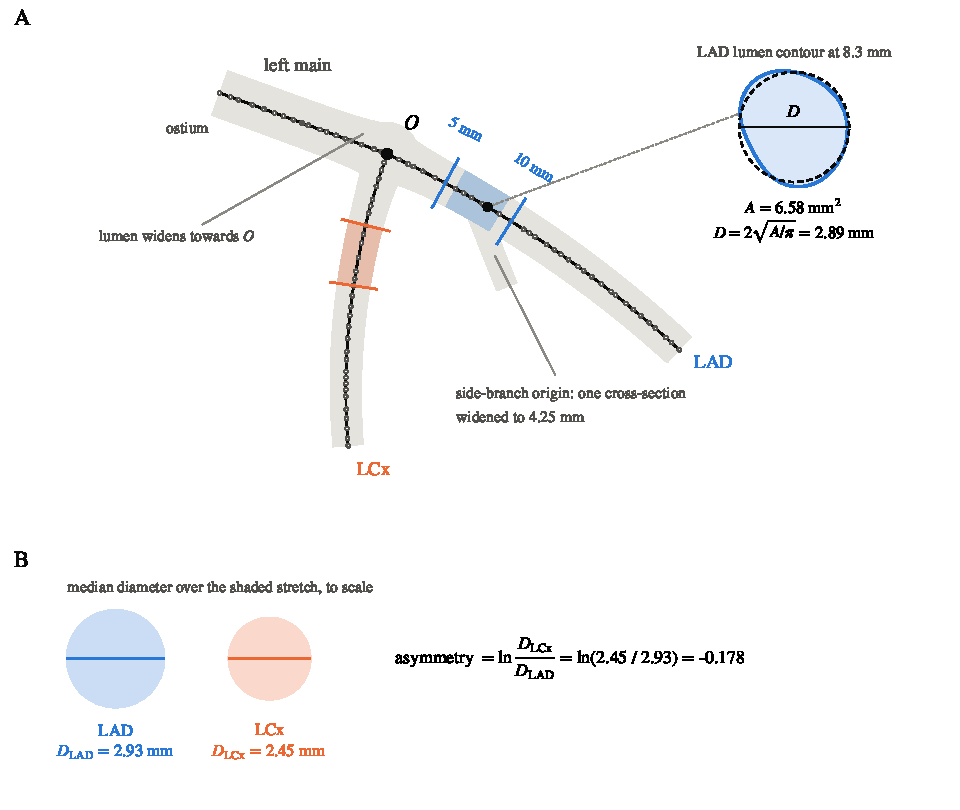
\includegraphics[width=\textwidth]{content/methodology/figures/daughter_ratio_figure.pdf}
  \caption{Daughter asymmetry on a made-up left main bifurcation, computed with the thesis code. Each lumen contour is reduced to the diameter $D$ of the circle with the same area, and the LAD and the LCx each to the median of $D$ over the shaded stretch 5 to 10\,mm from the bifurcation point $O$, which leaves out the widened lumen near $O$ and is not moved by the one cross-section widened at a side-branch origin (A). The two diameters, drawn to scale, give the daughter asymmetry (B).}
  \label{fig:method-ratio}
\end{figure}
